\chapter{Entscheidungsbaum}
\label{chap:entscheidungsbaum}

\begin{myremark}[Algorithmusart in diesem Kapitel]
    Funktionsart: \textbf{Klassifikation}. \\
    Umsetzungsart: \textbf{selbstlernend}, aber als Regelwerk gut nachvollziehbar.
\end{myremark}

\begin{myremark}
    Der Entscheidungsbaum ist einer der \textbf{intuitivsten} ML-Algorithmen:
    Er stellt Entscheidungen als Baumstruktur dar und ist leicht zu interpretieren.
\end{myremark}

\section{Grundidee}

\begin{mydefinition}[Entscheidungsbaum]
    Ein \textbf{Entscheidungsbaum} teilt Daten schrittweise auf.
    Jede \textbf{innere Knoten} stellt eine Frage (z.\,B. \enquote{Lernzeit > 6\,h?}),
    jede \textbf{Kante} führt zu einer Teilmenge, und jedes \textbf{Blatt} gibt
    die vorhergesagte Klasse an.
\end{mydefinition}

\begin{figure}[H]
    \centering
    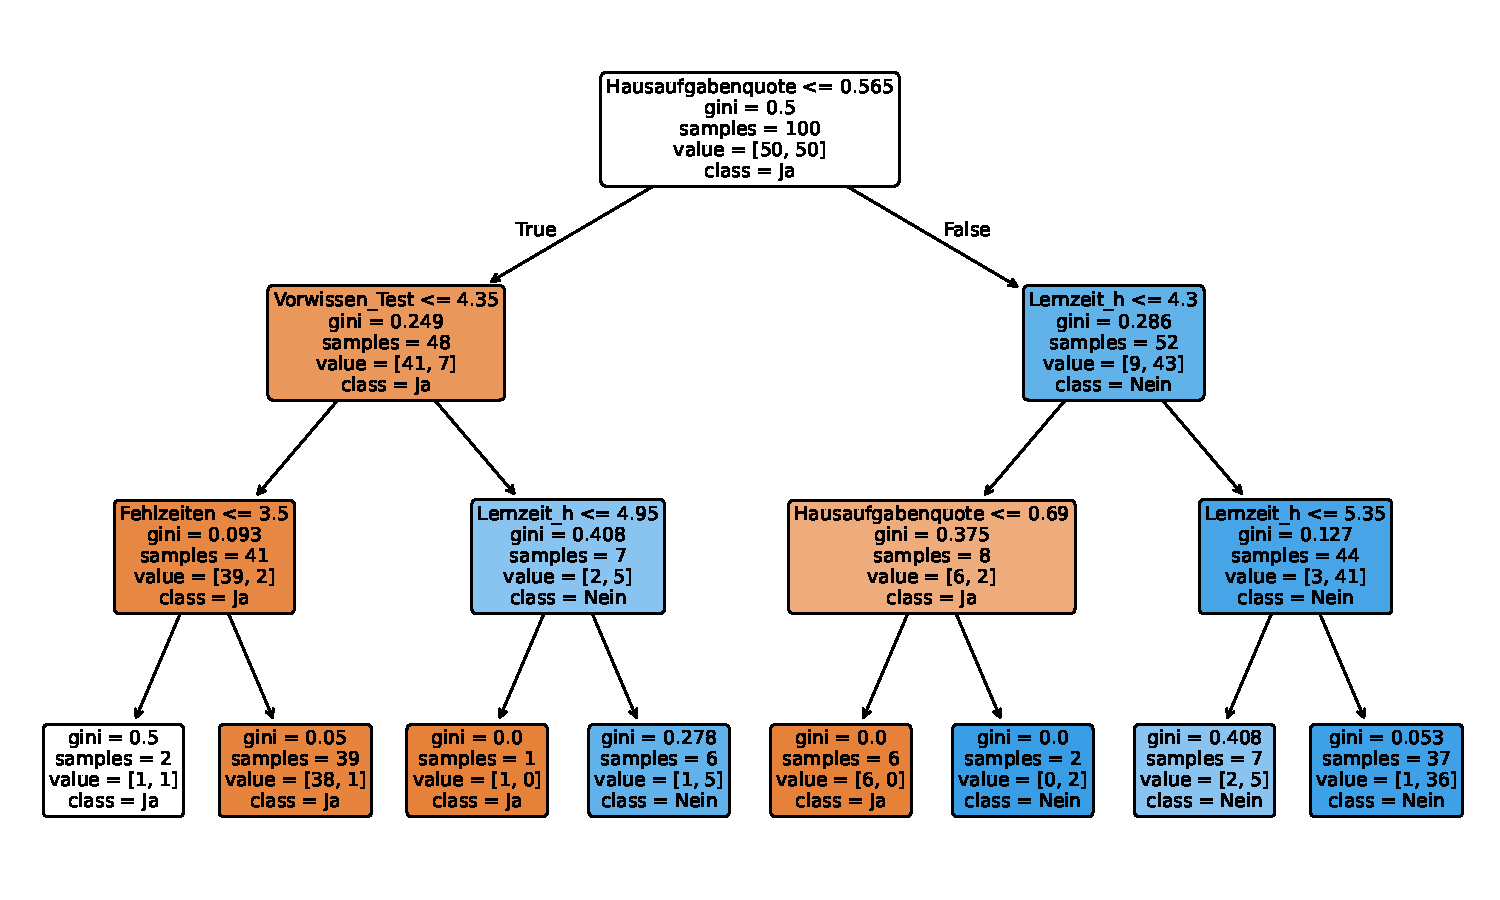
\includegraphics[width=0.8\textwidth]{Grundlagen_Info/10_KI_und_Algorithmen/Figures/decision_tree_structure.pdf}
    \caption{Beispiel eines Entscheidungsbaums}
    \label{fig:tree-15}
\end{figure}

\section{Wie lernt ein Baum?}

Ein Baum wählt an jedem Knoten jene Frage, die die Daten am besten aufteilt. Dabei sollte die Aufteilung möglichst \textbf{reine} Blätter erzeugen, d.\,h. Blätter, in denen die meisten Datenpunkte zur selben Klasse gehören. Als Gütemass wird häufig der \textbf{Gini-Koeffizient} verwendet:
\[
    \begin{aligned}
        \text{Gini}(t) & = 1 - (p_1^2 + p_2^2 + \cdots + p_k^2) \\
                       & = 1 - \sum_{k=1}^K p_k^2
    \end{aligned}
\]

wobei $p_k$ der Anteil der Klasse $k$ im Knoten $t$ ist.
Ein Gini von 0 bedeutet: alle Datenpunkte gehören zur selben Klasse (\enquote{reiner} Knoten). Um den Gini-Koeffizienten an jeder möglichen Aufteilung zu berechnen, muss der Algorithmus alle Features und Schwellenwerte durchprobieren -- das kann bei vielen Features und Datenpunkten sehr rechenintensiv sein. Deshalb werden oft Heuristiken oder Einschränkungen (z.\,B. maximale Tiefe) verwendet, um die Suche zu beschleunigen.


\begin{myexercise}[Gini-Koeffizienten von Hand berechnen]
    Betrachten Sie folgende Tabelle, die die Verteilung von Klassen in einem Knoten zeigt:
    \begin{center}
        \begin{tabular}{lcc}
            \toprule
            Klasse & Anzahl & Anteil $p_k$ \\
            \midrule
            A      & 40     & 0.4          \\
            B      & 30     & 0.3          \\
            C      & 20     & 0.2          \\
            D      & 10     & 0.1          \\
            \bottomrule
        \end{tabular}
    \end{center}
    Berechnen Sie den Gini-Koeffizienten für diesen Knoten.
    \begin{myanswer}
        \[
            \text{Gini} = 1 - (0.4^2 + 0.3^2 + 0.2^2 + 0.1^2) = 1 - (0.16 + 0.09 + 0.04 + 0.01) = 1 - 0.30 = 0.70
        \]
    \end{myanswer}
\end{myexercise}

\begin{myexercise}[Bestimmen der besten Aufteilung]
    Angenommen, Sie haben ein Feature \texttt{Lernzeit} mit den Werten $\{2, 4, 6, 8, 10\}$ Stunden und die folgenden Klassenlabels:
    \begin{center}
        \begin{tabular}{cc}
            \toprule
            Lernzeit (h) & Bestanden \\
            \midrule
            2            & nein      \\
            4            & nein      \\
            6            & ja      \\
            8            & ja      \\
            10           & ja      \\
            \bottomrule
        \end{tabular}
    \end{center}
    Zur Einfachheit nennen wir die Klassen \enquote{nein} als Klasse A und \enquote{ja} als Klasse B. Berechnen Sie den Gini-Koeffizienten für die Aufteilung bei $Lernzeit < 5$ und $Lernzeit < 7$ und bestimmen Sie, welche Aufteilung besser ist.
    
    \begin{myanswer}
        \begin{itemize}
            \item Für $Lernzeit < 5$:
            \begin{itemize}
                \item Links: Klasse A (2 Punkte), Gini = $1 - (1^2) = 0$
                \item Rechts: Klasse B (3 Punkte), Gini = $1 - (1^2) = 0$
                \item Gesamter Gini = $(5/5) * 0 + (0/5) * 0 = 0$
            \end{itemize}
            \item Für $Lernzeit < 7$:
            \begin{itemize}
                \item Links: Klasse A (2 Punkte), Klasse B (1 Punkt), Gini = $1 - (2/3)^2 - (1/3)^2 = 1 - (4/9 + 1/9) = 1 - 5/9 = 4/9$
                \item Rechts: Klasse B (2 Punkte), Gini = $1 - (1^2) = 0$
                \item Gesamter Gini = $(3/5) * (4/9) + (2/5) * 0 = (12/45) + 0 = 4/15$
            \end{itemize}
            \item Die Aufteilung bei $Lernzeit < 5$ ist besser, da sie einen niedrigeren Gini-Koeffizienten von $0$ im Vergleich zu $4/15$ hat.
        \end{itemize}
    \end{myanswer}
\end{myexercise}

\section{Overfitting}

\begin{myattention}
    Ein Baum ohne Tiefenbeschränkung \enquote{lernt} die Trainingsdaten auswendig --
    er kann jeden einzelnen Punkt korrekt klassifizieren, versagt aber bei neuen Daten.
    Dieses Phänomen heisst \textbf{Overfitting}.
\end{myattention}

\begin{mydefinition}[Overfitting und Underfitting]
    \begin{itemize}
        \item \textbf{Overfitting:} Modell ist zu komplex, lernt Rauschen im Trainingsset.
        \item \textbf{Underfitting:} Modell ist zu einfach, erkennt echte Muster nicht.
    \end{itemize}
\end{mydefinition}

\begin{myexercise}[Overfitting erkennen]
    Ein Modell erreicht auf den Trainingsdaten 99\,\% Accuracy,
    aber auf den Testdaten nur 62\,\%.
    \begin{enumerate}
        \item Liegt Overfitting oder Underfitting vor? Begründen Sie.
        \item Welcher Hyperparameter des Entscheidungsbaums kann Overfitting verringern?
    \end{enumerate}
    \begin{myanswer}
        1.\ Overfitting: sehr gute Trainings-, aber schlechte Testperformance. \\
        2.\ \texttt{max\_depth} begrenzt die Baumtiefe und verhindert überangepasste Modelle.
    \end{myanswer}
\end{myexercise}

\section{Gesellschaftliche Aspekte: Bias in Entscheidungsbäumen}

\begin{mydefinition}[Interpretierbarkeit als Doppelschwert]
    Obwohl Entscheidungsbäume besonders erklärbar sind, können vereinfachte Splits zu systematischen Verzerrungen führen. Dies gilt insbesondere dann, wenn Trainingsdaten strukturelle Diskriminierungen widerspiegeln oder wenn wichtige Kontextvariablen fehlen.
\end{mydefinition}

\begin{myexample}[Credit Scoring mit Entscheidungsbaum]
    Eine Bank verwendet einen Entscheidungsbaum zur Kreditvergabe. Ein historischer Split könnte sein: \enquote{Zip-Code < 50000?} Wenn bestimmte Stadtteile historisch benachteiligt wurden, führt diese geografische Variable zu unverhältnismässiger Ablehnung. Das Modell lernt und perpetuiert historische Diskriminierung, auch wenn nicht explizit nach Geschlecht oder Ethnie gefragt wird.

    \textbf{Real-World-Link:} \href{https://en.wikipedia.org/wiki/Redlining}{Redlining und strukturelle Diskriminierung in Credit Scoring}
\end{myexample}

\begin{mychallenge}[Bias durch vereinfachte Splits]
    Stellen Sie sich vor, Sie trainieren einen Entscheidungsbaum, um zu entscheiden, ob Kandidaten zu einem Bewerbungsgespräch eingeladen werden.
    Die Trainingsdaten stammen aus Ihrem Unternehmen der letzten 10 Jahre.
    \begin{enumerate}
        \item Welche versteckten Variablen könnten in historischen Einstellungsdaten kodiert sein?
        \item Wie könnte ein Split wie \enquote{Universität aus Top-20-Ranking?} zu Verzerrung führen?
        \item Welche Massnahmen könnten helfen, Bias beim Datensammlungs-Prozess zu reduzieren?
    \end{enumerate}
    \begin{myanswer}
        \begin{enumerate}
            \item Geschlecht, kultureller Hintergrund, sozioökonomischer Status (indirekt durch Universität, Wohnort, etc.).
            \item Wenn zu wenige Absolvent*innen von kleineren oder internationalen Universitäten historisch eingestellt wurden, reproduziert das Modell diese Ungleichheit.
            \item Bewusste Datensammlung von unterrepräsentierten Gruppen, regelmässige Bias-Audits, oder explizite Fairness-Constraints beim Trainieren des Baums.
        \end{enumerate}
    \end{myanswer}
\end{mychallenge}

\begin{myremark}[Notebook]
    Praktische Umsetzung inkl. Übungen:
    \href{\notebookbaseurl01_Entscheidungsbaum_Classification.ipynb}{\texttt{01\_Entscheidungsbaum.ipynb}}
\end{myremark}
